%% limitations.tex - Many-one and kernel reductions differ
%%
%% Copyright 2014 Jeffrey Finkelstein.
%%
%% This LaTeX markup document is made available under the terms of the Creative
%% Commons Attribution-ShareAlike 4.0 International License,
%% https://creativecommons.org/licenses/by-sa/4.0/.
\section{Limitations of kernel reductions}\label{sec:limitations}
% Foreword
%
% context (focus on anyone) why now? - current situation, and why the need is so important
Can a kernel reduction be used anywhere a many-one reduction can be used?
% need (focus on readers) why you? - why this is relevant to the reader, and why something needed to be done
If so, a function with access to one element of a pair would be exactly as powerful as a function with access to both elements of a pair; our intuition is that this is unlikely.
% task (focus on author) why me? - what was undertaken to address the need
% object (focus on document) why this document - what the document covers
This section proves that polynomial time kernel reductions are strictly weaker than polynomial time many-one reductions.

% Summary
%
% findings (focus on author) what? - what the work revealed when performing the task
We discovered that a bound on the size of the image of a kernel reduction implies that the function can only access a finite number of equivalence classes.
Constructing equivalence relations so that there is an imbalance in the number of equivalence classes with respect to any fixed function suffices to show that no polynomial time kernel reduction can exist between the two.
% conclusion (focus on readers) so what? - what the findings mean for the audience
As a more restrictive type of reduction and hence as a finer-grained tool for comparing the relative difficulty of equivalence problems, kernel reductions should be used when proving a reduction (if one exists) between equivalence problems.
% perspective (focus on anyone) what now? - what should be done next
This will be important for \autoref{sec:generalcompleteness} as well, since it means that completeness under kernel reductions is distinct from completeness under many-one reductions.

We adopt and extend the notation $\#R$, from \autocite{bcffm}, to denote the number of equivalence classes in an equivalence relation $R$.

\begin{definition}[{\autocite[Section~5]{bcffm}}]%Definition~7.2]{bcffm}}]
  Suppose $R$ is an equivalence relation on $\Sigma^*$.
  Let $\#R(n) = \left|\left\{[x]_R \, \middle| \, x \in \Sigma^{\leq n}\right\}\right|$, or in other words, $\#R(n)$ is the number of equivalence classes in $R$ for strings of length at most $n$.
  Let $\#R = \max\limits_{n \in \mathbb{N}} \#R(n)$ if the maximum exists, or in other words, $\#R$ is the number of equivalence classes in $R$.
\end{definition}

As first stated in \autocite{fg11}, if the number of equivalence classes in $R$ is greater than the number of equivalence classes in $S$, then no kernel reduction can exist (regardless of any time or space bounds on the function computing the reduction).
For completeness, we prove this basic fact in \autoref{prop:noreduction} below.
However, a many-one reduction can overcome this restriction by having access to both strings in the pair.
Before proving that, we require the following lemma showing that kernel reductions must preserve ``related-ness'' of pairs of elements by mapping equivalence classes in $R$ to equivalence classes in $S$.

\begin{lemma}\label{lem:image}
  Suppose $R$ and $S$ are equivalence relations on $\Sigma^*$.
  Suppose $R \krnt S$ and $f$ is the function computing the kernel reduction.
  Let $\hat{f}$ denote the function defined by $\hat{f}([x]_R) = [f(x)]_S$, for all equivalence classes $[x]_R$ in $R$.
  Then the following are true.
  \begin{itemize}
  \item $\hat{f}$ is injective
  \item $f([w]_R) \subseteq \hat{f}([w]_R)$ for any $w \in \Sigma^*$
  \end{itemize}
\end{lemma}
\begin{proof}
  First, we prove that $\hat{f}$ is injective.
  Let $[x]_R$ and $[y]_R$ be distinct equivalence classes in $R$.
  Suppose $\hat{f}([x]_R) = \hat{f}([y]_R)$, so $[f(x)]_S = [f(y)]_S$.
  In other words, $\pair{f(x)}{f(y)} \in S$.
  By definition of the kernel reduction $f$, this implies $\pair{x}{y} \in R$.
  Therefore $[x]_R = [y]_R$.

  Next, we prove that $f([w]_R) \subseteq \hat{f}([w]_R)$.
  Since $w \in [w]_R$, it follows that $f(w) \in f([w]_R)$.
  Let $x \in f([w]_R)$.
  Then $\pair{x}{f(w)} \in S$, so $x \in [f(w)]_S$.
  Therefore $f([w]_R) \subseteq [f(w)]_S = \hat{f}([w]_R)$.
\end{proof}

\begin{proposition}\label{prop:noreduction}
  Let $R$ and $S$ be equivalence relations on $\Sigma^*$.
  If $\#R > \#S$, then $R \nkrnt S$.

  Furthermore, suppose $\#R = n$ and $\#S = m$, and suppose $m \geq 2$.
  Let $r_1, \dotsc, r_n$ and $s_1, \dotsc, s_m$ denote representatives of the equivalence classes in $R$ and $S$, respectively.
  If the problem of deciding whether $x \in [r_i]_R$ for any $x \in \Sigma^*$ is recognizable, then $R \mornt S$.
\end{proposition}
\begin{proof}
  Assume that $R \krnt S$.
  By \autoref{lem:image}, the function mapping equivalence classes in $R$ to equivalence classes in $S$ induced by the kernel reduction is injective.
  However, this violates the pigeonhole principle.
  Therefore no kernel reduction exists from $R$ to $S$.

  On the other hand, there is a many-one reduction from $R$ to $S$.
  First, suppose $S$ has $m$ equivalence classes and let $s_1, \dotsc, s_m$ be representatives of each equivalence class in $S$.
  On input $\pair{x}{y}$, for each $i \in \{1, \dotsc, n\}$ in parallel, determine if $x \in [r_i]_R$ and $y \in [r_i]_R$ (also in parallel).
  If $x$ and $y$ are both in $[r_i]_R$ for some $i$, output $\pair{s_i}{s_i}$, otherwise output $\pair{s_1}{s_2}$.

  Since each string must be in exactly one of the equivalence classes of $R$, this function must halt when searching for the equivalence class for the strings $x$ and $y$.
  If $\pair{x}{y} \in R$, then they are in the same equivalence class of $R$ and hence the function will output $\pair{s_i}{s_i}$, which is in $S$ by the reflexivity of $S$.
  If $\pair{x}{y} \notin R$, then they are in different equivalence classes and hence the function will output $\pair{s_1}{s_2}$, which is not in $S$ because $[s_1]_S \neq [s_2]_S$ by hypothesis.
  Therefore this function is a computable many-one reduction from $R$ to $S$.
\end{proof}

\begin{example}
  Let $R = \mathbb{Z} / 3 \mathbb{Z}$ and $S = \mathbb{Z} / 2 \mathbb{Z}$.
  Then $R \mornt S$ but $R \nkrnt S$.
\end{example}

As seen in \autoref{prop:noreduction}, for equivalence relations $R$ and $S$ with a finite number of equivalence classes, a kernel reduction from $R$ to $S$ can only exist if the number of equivalence classes in $R$ is at most the number of equivalence classes in $S$.
However, most ``interesting'' equivalence relations have an infinite number of equivalence classes.
In \autocite[Section~4]{fg11}, the authors ask if there are such equivalence relations ``of the same densities [that is, density of equivalence classes] on which kernel reduction and [many-one] reduction differ''.
\autocite[Theorem~5.1]{bcffm} (see also \autocite[Remark~5.2]{bcffm}) answers this question affirmatively, providing an infinite antichain of equivalence relations that are equivalent under polynomial time many-one reductions but otherwise incomparable under polynomial time ``strong isomorphism reductions'' (proven in \autocite[Section~7]{bcffm} to be equivalent to polynomial time kernel reductions).
We will provide a simple proof of a special case of \autocite[Theorem~5.1]{bcffm}, showing that an imbalance in the density of equivalence classes prevents a kernel reduction.
This proof is valuable because it requires only knowledge of basic computational complexity theory and not knowledge of Boolean algebras, descriptive set theory, or other mathematical logic.

First we show that an equivalence relation dense in equivalence classes cannot be reduced to one sparse in equivalence classes.
We emphasize that our result does not concern the sparseness of strings in a language, but the sparseness of equivalence classes in an equivalence relation.
This complements the work on ``potential reducibility'' defined in \autocite[Section~5]{bcffm}.

\begin{definition}[{\autocite[Definition~7.2]{bcffm}}]
  Let $R$ and $S$ be equivalence relations on $\Sigma^*$.
  $R$ is \defn{potentially reducible} to $S$, denoted $R\pot S$, if there exists a polynomial $p$ such that for all $n\in\mathbb{N}$, $\#R(n)\leq \#S(p(n))$.
\end{definition}

It follows from the definitions that for any equivalence relations $R$ and $S$, $R\kr S\implies R\pot S$, and hence $R\npot S \implies R\nkr S$ (this is stated and proven explicitly in \autocite[Lemma~5.5]{bcffm}).
As an analog to traditional sparse languages, we provide a definition of ``kernel sparsity'', and show its application to determining potential reducibility and hence kernel reducibility.

\begin{definition}
  An equivalence relation $R$ on $\Sigma^*$ is \defn{kernel sparse} if there exists a polynomial $p$ such that for all $n\in\mathbb{N}$, $\#R(n)\leq p(n)$.
  In other words, the number of equivalence classes in $R$ for strings of length at most $n$ is bounded above by a polynomial in $n$.

  An equivalence relation is \defn{kernel dense} if it is not kernel sparse.
  Formally, if for all polynomials $p$ there exists an $n\in\mathbb{N}$ such that $\#R(n)>p(n)$.
  In other words, the number of equivalence classes in $R$ for strings of length at most $n$ is greater than any polynomial in $n$.
\end{definition}

These definitions allow us to provide the following very natural proposition.
Intuitively, it states that an equivalence relation with many closely packed equivalence classes cannot reduce (under polynomially bounded notions of reduction) to an equivalence relation with few but widely spaced equivalence classes.
This is essentially a special case of \autocite[Lemma~2.3]{gz14}.

\begin{theorem}\label{thm:density}
  Let $R$ and $S$ be equivalence relations on $\Sigma^*$.
  If $R$ is kernel dense and $S$ is kernel sparse, then $R\nkr S$.
\end{theorem}
\begin{proof}
  That $R\npot S$ implies $R\nkr S$ was already stated in the text preceding this theorem, so it suffices to show that $R\npot S$.

  Assume that $R\pot S$ with the intention of producing a contradiction.
  Let $p$ be the polynomial such that $\#R(n)\leq \#S(p(n))$ (this is the definition of potential reducibility).
  Let $q$ be the polynomial such that for all $n$, $\#S(n)< q(n)$ (this is the definition of kernel sparse).
  %% TODO is this true?
  Assume without loss of generality that $q$ is non-decreasing (we can do this because for each polynomial $a$ there exists a non-decreasing polynomial $b$ such that $a(n)\leq b(n)$ for all $n$).
  For each natural number $n$, we have $\#S(n) \leq q(0) + q(1) + \cdots + q(n) \leq n \cdot q(n)$ (since $q$ is non-decreasing).
  Replacing $n$ with $p(n)$ in the above inequality, it follows that $\#S(p(n)) \leq p(n) \cdot q(p(n))$, which is a polynomial in $n$.
  (This is an overestimate, but we can be generous here and still produce a contradiction.)
  Let $r(n)=p(n)\cdot q(p(n))$.

  Let $n_0$ be the natural number such that $\#R(n_0) > r(n_0)$, by the definition of kernel sparse.
  Since $\#S(p(n_0)) \leq r(n_0)$, we have $\#R(n_0) > \#S(p(n_0))$.
  In other words, there are more equivalence classes in $R$ for strings up to length $n_0$ than there are in $S$ for strings up to length $p(n_0)$.
  By the pigeonhole principle, we conclude that $R$ cannot potentially reduce to $S$, because the number of equivalence classes in $R$ for strings up to length $n_0$ is too great compared to the number of equivalence classes in $S$ for strings up to length $p(n_0)$.
  This is a contradiction with the assumption that $R\pot S$.
  We have shown this for arbitrary polynomials (which came from the definitions of potential reducibility and kernel sparsity), so we can conclude that the result holds for all equivalence relations $R$ and $S$ which are kernel dense and kernel sparse, respectively.
\end{proof}

\begin{example}
  Consider the equality relation and the ``equal lengths'' relation (that is, $x$ relates to $y$ if $|x| = |y|$).
  The equality relation is kernel dense, since there are $2^n$ equivalence classes for strings of length at most $n$ (one for each string).
  The ``equal lengths'' relation is kernel sparse, since there are $n + 1$ equivalence classes for strings of length at most $n$ (one for each length, including length $0$).
  Therefore there is no polynomial time kernel reduction from the equality relation to the ``equal lengths'' relation.
\end{example}

This places a strong restriction on equivalence relations which are hard (or complete) under polynomial time kernel reductions: they cannot be kernel sparse.

\begin{corollary}
  Let $\CEq$ be a complexity class of equivalence relations containing the equality relation $R_{eq}$.
  If an equivalence relation $R$ is kernel sparse, then it is not $\CEq$-hard.
\end{corollary}
\begin{proof}
  $R_{eq}$ is kernel dense since it contains $2^n$ equivalence classes at each length $n$, one for each distinct string.
  Since $R$ is kernel sparse, then $R_{eq} \nkr R$ by \autoref{thm:density}.
  Since $R_{eq} \in \CEq$, the equivalence relation $R$ cannot be $\CEq$-hard.
\end{proof}

Polynomial time many-one reductions are more powerful than polynomial time kernel reductions, because the former are not subject to restrictions on numbers of equivalence classes as in \autoref{prop:noreduction} and \autoref{thm:density}.
The idea behind \autoref{thm:density} leads to a construction of equivalence relations $R$ and $S$ between which there is a polynomial time many-one reduction but no polynomial time kernel reduction.

\begin{construction}\label{con:rands}
  Let $f_1, f_2, \dotsc$ be an enumeration of all polynomial time computable functions.
  Assume without loss of generality \todo{state why} that for all positive integers $i$, function $f_i$ runs in time $p_i(n)$, where $p_i(n) = i n^i$ for all positive integers $n$.

  Suppose $n$ is a positive integer.
  Define $R_n$ as the set of all strings of length $n$, except $R_1$, which also includes the string of length $0$.
  Define $S_n$ as the set of all strings $s$ satisfying the inequality $p_n(n) + 1 \leq |s| \leq p_{n + 1}(n + 1)$, except $S_1$, which includes all strings of length at most $p_2(2)$.

  Define sets $R$ and $S$ as
  \begin{equation*}
    R = \bigcup_{n \in \mathbb{Z}^+} R_n \times R_n \text{ and } S = \bigcup_{n \in \mathbb{Z}^+} S_n \times S_n.
  \end{equation*}
\end{construction}

\begin{lemma}
  $R$ and $S$ are equivalence relations.
\end{lemma}
\begin{proof}
  $R$ and $S$ are equivalence relations if $\{R_n\}_{n \in \mathbb{Z}^+}$ and $\{S_n\}_{n \in \mathbb{Z}^+}$ are valid partitions of $\Sigma^*$, so it suffices to show that each set in the collection is nonempty, the union of each collection includes all nonempty strings in $\Sigma^*$, and each collection is pairwise disjoint.

  The set $R_n$ includes at least one string of length $n$, so each $R_n$ is nonempty.
  Any string of length $n$ is in $R_n$, so $\Sigma^* \subseteq \cup_n R_n$.
  If $m$ and $n$ are distinct positive integers, no string can have both length $m$ and length $n$, so $R_m \cap R_n = \emptyset$.
  Hence $\{R_n\}_n$ is a valid partition.

  We need to show $p_n(n) + 1 \leq p_{n + 1}(n + 1)$ in order to prove that there is at least one string (of length $p_n(n) + 1$, for example) in $S_n$.
  \begin{align*}
    p_n(n) + 1 &= n (n^n) + 1 \\
    &\leq n (n^n) + n^n \\ %% && \text{(since } 1 \leq n^n \text{ for each } n \text{)} \\
    &= (n + 1) n^n \\
    &\leq (n + 1) (n + 1)^{n + 1} \\
    &= p_{n + 1}(n + 1).
  \end{align*}
  Thus there is at least one string in $S_n$.
  Next, for any string $x$, there exists an $n$ such that $p_n(n) + 1 \leq |x| \leq p_{n + 1}(n + 1)$, so every string in $\Sigma^*$ is in some $S_n$.
  \todo{I don't know how to explain this further.}
  Finally, suppose $m$ and $n$ are distinct positive integers and assume without loss of generality that $m < n$, or in other words, that $m + 1 \leq n$.
  Then $p_{m + 1}(m + 1) \leq p_n(n) < p_n(n) + 1$, so no string of length at most $p_{m + 1}(m + 1)$ can also have length at least $p_n(n) + 1$.
  Hence, $S_m$ and $S_n$ are disjoint.
  Thus, $\{S_n\}_n$ is a valid partition.

  Since both collections are valid partitions, the relations $R$ and $S$ are both equivalence relations.
\end{proof}

Again, this is a special case of \autocite[Theorem~5.1]{bcffm}, but has a much simpler proof and sufficiently demonstrates that polynomial time kernel reductions and polynomial time many-one reductions are different.

\begin{theorem}\label{thm:different}
  There are equivalence relations $R$ and $S$ such that $R \mor S$ but $R \nkr S$.
  Furthermore, $R$ and $S$ are in $\NC^1$.
\end{theorem}

\begin{figure}
  \caption{\label{fig:sparse}For a fixed kernel reduction $f_n$ running in time $p_n$, the image of a string of length $n + 1$ can only be a string of length at most $p_n(n + 1)$.
    The number of equivalence classes in $R$ for strings of length $n + 1$ is greater than the number of equivalence classes in $S$ for strings of length $p_n(n + 1)$ for each polynomial $p_n$.}
  \begin{center}
    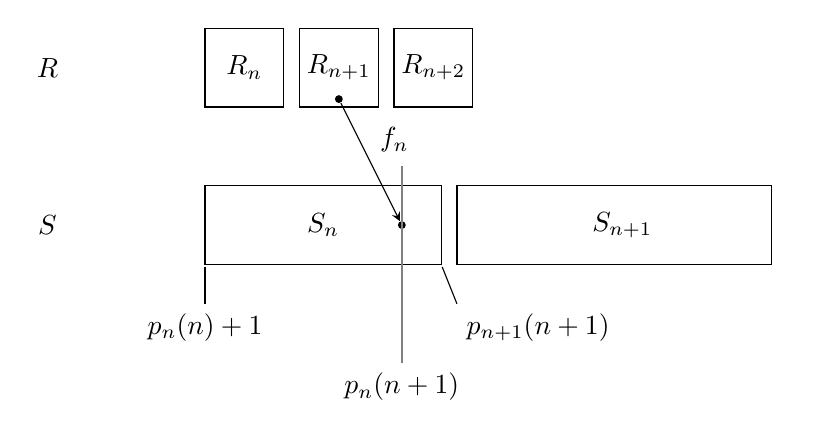
\begin{tikzpicture}[yscale=0.5]
      \begin{scope}[shift={(0, 5)}]
        \node at (0, 1) {$R$};

        %% Rectangles for equivalence classes of $R$.
        \draw (2, 0)
        %% TODO should be a way to use [current node is local] option here...
        ++(0, 1) node[anchor=east] {$\dotsb$} ++(0, -1)
        rectangle ++(1, 2)
        ++(0.2, -2)
        rectangle ++(1, 2)
        ++(0.2, -2)
        rectangle ++(1, 2)
        ++(0, -1)
        node[anchor=west] {$\dotsb$}
        ;

        %% Labels for each equivalence class of $R$.
        \path
        (2.5, 1) node {$R_n$}
        ++(1.2, 0) node {$R_{n + 1}$}
        ++(1.2, 0) node {$R_{n + 2}$}
        ;
      \end{scope}

      %% Arrow from top to bottom showing image under $f_n$.
      \begin{scope}[shift={(0, 1)}]
        \draw
        (4.5, 1) node[shape=circle, fill=black, inner sep=1pt] (source) {}
        ++(-0.8, 3.2) node[shape=circle, fill=black, inner sep=1pt] (target) {};
        \path[<-, >=stealth] (source) edge node[anchor=south west] {$f_n$} (target);
      \end{scope}

      \begin{scope}[shift={(0, 1)}]
        \node at (0, 1) {$S$};

        %% Rectangles for equivalence classes of $S$.
        \draw (2, 0)
        %% TODO should be a way to use [current node is local] option here...
        ++(0, 1) node[anchor=east] {$\dotsb$} ++(0, -1)
        rectangle ++(3, 2)
        ++(0.2, -2)
        rectangle ++(4, 2)
        ++(0, -1)
        node[anchor=west] {$\dotsb$}
        ;

        %% Labels for each equivalence class of $S$.
        \path
        (3.5, 1) node {$S_n$}
        ++(3.8, 0) node {$S_{n + 1}$}
        ;
      \end{scope}

      %% Labels underneath each $S_i$ showing length bounds.
      \begin{scope}
        \draw[shorten >=1pt]
        (2, 0) node[anchor=north] (pn) {$p_n(n) + 1$}
        -- ++(0, 1);
        \draw[thick, color=gray] (4.5, 3.5)
        -- ++(0, -5)
        node[anchor=north, color=black] (pnplus1) {$p_n(n + 1)$}
        ;
        \draw[shorten >=1pt]
        (5.2, 0) node[anchor=north west, color=black] (pnplus1nplus1) {$p_{n + 1}(n + 1)$}
        -- ++(-0.2, 1);
        ;
      \end{scope}
    \end{tikzpicture}
  \end{center}
\end{figure}

The main idea behind this theorem is that no matter which polynomial time function we consider as a possible kernel reduction, the number of equivalence classes in $R$ is greater than the number of equivalence classes in $S$, for sufficiently large strings.
\autoref{thm:density} doesn't apply in this setting because both $R$ and $S$ are kernel sparse.
Since we have carefully constructed these sets, $S$ is more kernel sparse than $R$.
This basic idea was presented independently in \autocite[Lemma~2.3]{gz14}.

Though it is not explicitly stated here, this theorem can be generalized to kernel reductions with other (non-polynomial) time bounds in a straightforward manner.

\begin{proof}[Proof of \autoref{thm:different}]
  Let $R$ and $S$ be the equivalence relations in \autoref{con:rands}.
  The following function is a polynomial time many-one reduction from $R$ to $S$.
  On input $\pair{x}{y}$, if $|x| = |y|$ (or if $|x|$ and $|y|$ are both in $\{0, 1\}$), output $\pair{a}{a}$, otherwise output $\pair{a}{b}$, where $a$ is a string in $S_1$ and $b$ is a string in $S_2$.
  Computing and comparing the lengths of $x$ and $y$ can be done in linear time and writing the output requires only a constant number of steps, since the lengths of $a$ and $b$ are independent of the lengths of $x$ and $y$.
  Thus this function is computable in linear time, and hence in polynomial time.
  If $\pair{x}{y} \in R$, then the function outputs $\pair{a}{a}$, which is in $S$ since $S$ is reflexive.
  If $\pair{x}{y} \notin R$, then the function outputs $\pair{a}{b}$, which is not in $S$ since $a$ and $b$ are in different equivalence classes of $S$.
  Therefore there is a correct polynomial time many-one reduction from $R$ to $S$.

  Now assume with the intention of producing a contradiction that there is a polynomial time kernel reduction from $R$ to $S$.
  Since $f_1, f_2, \dotsc$ is an enumeration of all polynomial time computable functions, the reduction from $R$ to $S$ is $f_n$, with running time $p_n$, for some positive integer $n$.
  Consider a string $x$ of length $n + 1$ (for example, $x = 1^{n + 1}$); $x$ is in equivalence class $R_{n + 1}$.
  Since the running time of $f_n$ is $p_n$, the length of $f_n(x)$ is at most $p_n(n + 1)$.
  Since $p_1, p_2, \dotsc$ is an increasing sequence (in the sense that $p_j(n) < p_{j + 1}(n)$ for all natural numbers $n$ and all positive integers $j$), we have $p_n(n + 1) < p_{n + 1}(n + 1) < p_{n + 1}(n + 1) + 1$.
  %% The image of any string of length $n + 1$ has length at most $p_n(n + 1)$, which is strictly less than $p_{n + 1}(n + 1) + 1$.
  By the construction of $R$ and $S$, we have $\#R(n + 1) = n + 1$ and $\#S(p_n(n + 1)) \leq \#S(p_{n + 1}(n + 1)) = n$.
  By the pigeonhole principle, there must be two strings $x$ and $y$ of length at most $n + 1$ in different equivalence classes of $R$ whose image under $f_n$ is in the same equivalence class of $S$.
  Since $\pair{x}{y} \notin R$ if and only if $\pair{f(x)}{f(y)} \notin S$, this is a contradiction.
  Therefore $R \nkr S$.

  Finally, we show that $R$ and $S$ are in $\NC^1$.
  Deciding whether two strings have the same length is trivial, so $R$ is certainly in $\NC^1$.
  To decide $S$, we compute the index $i$ of the equivalence class $S_i$ containing the string $x$ and the index $j$ of the equivalence class $S_j$ containing the string $y$, then compare them for equality.
  Computing the index $i$ of the equivalence class of a string $x$ of length $n$ can be performed as follows.
  First, compute in parallel the values $p_1(1), \dotsc, p_{n + 1}(n + 1)$.
  Since each $p_i$ is increasing, $n$ is definitely smaller than $p_{n + 1}(n + 1)$.
  Computing the exponentiation of $O(n)$ pairs of strings of length $O(n)$ each can be performed by a $\TC^0$ circuit, and $\TC^0 \subseteq \NC^1$.
  Next, for each $i \in \{1, \dotsc, n\}$ in parallel, decide if $p_i(i) + 1 \leq n \leq p_{i + 1}(i + 1)$, thereby determining whether the input is in $S_i$.
  These comparisons can be performed by an $\NC^1$ circuit.
  Finally, use $O(\log n)$ single-bit multiplexers in parallel to output the index (in binary) of the sole equivalence class $S_i$ containing $x$.
  A single-bit multiplexer for $O(\log n)$ input bits can be implemented by a circuit of size $O(\log n)$ and depth $O(\log \log n)$ \autocite[Lemma~2.5.5]{savage98}, so this phase of the computation can be performed by an $\NC^1$ circuit.
  Computing the indices $i$ and $j$ for the two input strings can be performed in parallel, and the final comparison for equality of $i$ and $j$ adds only $O(\log n)$ depth to the circuit.
  Therefore $S \in \NC^1$.
\end{proof}
